
% =============================================================================
% Project : THE PHILOSOPHY OF VIABILITY
% Book    : Book I — Ontology of Viability
% Book ID : VS.B01
% Chapter : 08 — Comparative Philosophical Examination
% Section : 02 — Parmenides
%
% Asset ID:
%   VS.B01.P01.C08.S02.SS01.P003.IL01
%
% Type    : IL — Illustration
% File    : threshold_of_inquiry.tex
%
% Purpose :
%   Provide a restrained symbolic illustration of the threshold
%   imagery in the proem of Parmenides' poem. The image is
%   interpretive and atmospheric, not a historical reconstruction
%   or a diagram of the poem's philosophical argument.
% =============================================================================

\begin{figure}[htbp]
\centering

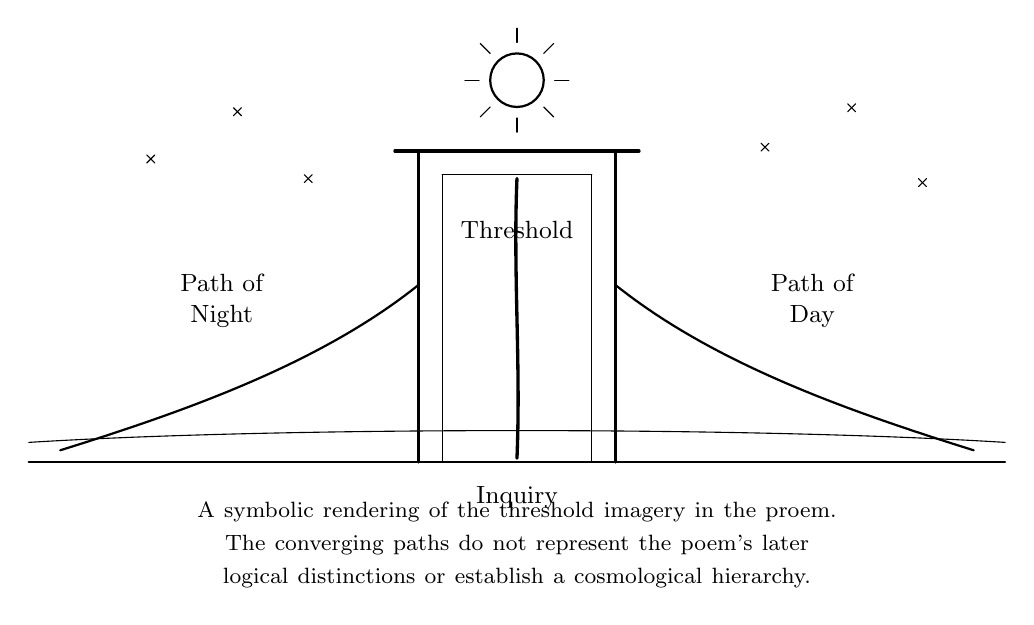
\begin{tikzpicture}[
    line cap=round,
    line join=round,
    scale=1.0
]

% Ground and horizon
\draw[thick] (-6.2,-2.4) -- (6.2,-2.4);
\draw[thin] (-6.2,-2.15) .. controls (-3.0,-1.95)
    and (3.0,-1.95) .. (6.2,-2.15);

% Threshold structure
\draw[very thick] (-1.25,-2.4) -- (-1.25,1.55);
\draw[very thick] (1.25,-2.4) -- (1.25,1.55);
\draw[very thick] (-1.55,1.55) -- (1.55,1.55);

% Inner gate lines
\draw[thin] (-0.95,-2.4) -- (-0.95,1.25);
\draw[thin] (0.95,-2.4) -- (0.95,1.25);
\draw[thin] (-0.95,1.25) -- (0.95,1.25);

% Two paths approaching the threshold
\draw[thick]
    (-5.8,-2.25)
    .. controls (-4.2,-1.75) and (-2.5,-1.15)
    .. (-1.25,-0.15);

\draw[thick]
    (5.8,-2.25)
    .. controls (4.2,-1.75) and (2.5,-1.15)
    .. (1.25,-0.15);

% Central path beyond the gate
\draw[very thick]
    (0,-2.35)
    .. controls (0.05,-1.15) and (-0.05,0.0)
    .. (0,1.2);

% Sun and stars
\draw[thick] (0,2.45) circle (0.34);
\foreach \a in {0,45,...,315}{
    \draw[thin]
        ({0.48*cos(\a)},{2.45+0.48*sin(\a)})
        --
        ({0.66*cos(\a)},{2.45+0.66*sin(\a)});
}

\foreach \x/\y in {-4.7/1.4,-3.6/2.0,-2.7/1.15,
                    3.1/1.55,4.2/2.05,5.1/1.1}{
    \draw[thin] (\x,\y) -- ++(0.10,0.10);
    \draw[thin] (\x+0.10,\y) -- ++(-0.10,0.10);
}

% Labels
\node[align=center] at (-3.75,-0.35)
    {\small Path of\\[-1pt]\small Night};

\node[align=center] at (3.75,-0.35)
    {\small Path of\\[-1pt]\small Day};

\node[align=center] at (0,0.55)
    {\small Threshold};

\node[align=center] at (0,-2.85)
    {\small Inquiry};

% Caption note within the illustration
\node[align=center,text width=10.5cm] at (0,-3.45)
    {\footnotesize
    A symbolic rendering of the threshold imagery in the proem.
    The converging paths do not represent the poem's later
    logical distinctions or establish a cosmological hierarchy.};

\end{tikzpicture}

\caption{The Threshold of Inquiry in the Proem of Parmenides}
\label{fig:ch08-parmenides-threshold}

\end{figure}

% =============================================================================
% END OF ASSET
% =============================================================================
